\section{Concepts}

\subsection{Operating Systems}

\begin{frame}{IT trends}
	\begin{itemize}
		\item More resources
			\begin{itemize}
			\item Better hardware at lower costs
			\item Higher standards for software quality
			\end{itemize}
		\item More users
			\begin{itemize}
			\item Contact with technology at an earlier age
			\item Shared access to the same device
			\end{itemize}
		\item Data consolidation
			\begin{itemize}
			\item Data warehousing
			\item Service unification
			\item Differentiated access
			\end{itemize}
		\item Increased flexibility
			\begin{itemize}
			\item Versatile configuration
			\item Focus on usability
		\end{itemize}
	\end{itemize}
\end{frame}

\begin{frame}{OS Recap}
	\begin{columns}[T]
		\begin{column}{.5\textwidth}
			\begin{itemize}
			\item Resources
				\begin{itemize}
				\item CPU
				\item Memory
				\item Peripherals
				\end{itemize}
			\item Structures
				\begin{itemize}
				\item The scheduler
				\item The pager
				\item Filesystems
				\end{itemize}
			\item The kernel
				\begin{itemize}
				\item Handles hardware
				\item Exposes capabilities
				\item Manages resources
				\end{itemize}
			\end{itemize}
		\end{column}
		\begin{column}{.5\textwidth}
			\begin{figure}[ht]
				\vspace*{-0.7cm}
				\caption{The Memory Pager}
				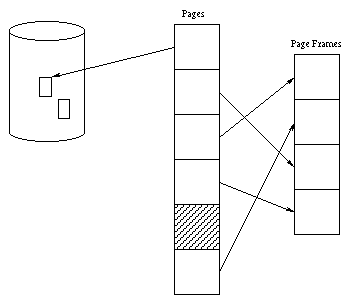
\includegraphics[height=0.3\textheight]{img/pager.png}
			\end{figure}
			\begin{figure}[ht]
				\vspace*{-0.7cm}
				\caption{The Scheduler}
				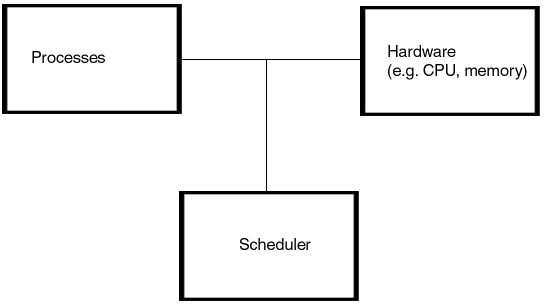
\includegraphics[height=0.3\textheight]{img/scheduler.png}
			\end{figure}
		\end{column}
	\end{columns}
\end{frame}

\subsection{Virtualization}

\begin{frame}{Virtualization}
	\begin{columns}[T]
		\begin{column}{.6\textwidth}
			\begin{itemize}
			\item Key aspects:
				\begin{itemize}
				\item Simulation (of HW / SW)
				\item Virtual machines
				\item Autonomous computing
				\item Utility computing
				\end{itemize}
			\item Advantages:
				\begin{itemize}
				\item Better resource usage
				\item Lower running costs
				\item Improved security
				\end{itemize}
			\item Concerns:
				\begin{itemize}
				\item Management
				\item Isolation
				\item Performance
				\item Applicability
				\end{itemize}
			\end{itemize}	
		\end{column}
		\begin{column}{.4\textwidth}
			\begin{figure}[hb]
				\centering
				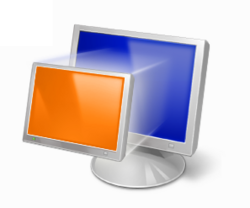
\includegraphics[width=\textwidth]{img/virt.png}
			\end{figure}
		\end{column}
	\end{columns}
\end{frame}

\begin{frame}{OS-level Virtualization}
	\begin{itemize}
	\item One host
	\item Multiple running OS instances
	\item Rootfs, system libs, binaries
	\end{itemize}
	
	OS instance = a process hierarchy
	
	OS level virtualization = \textbf{partitioning} the process tree
	
	Advantage: \textbf{close to 0\% performance overhead}
	
	Flaw: \textbf{shared kernel}
\end{frame}